\section{System Architecture and Design}

Figure~\ref{fig:architect} shows an overview design of our system. The components of the system is discussed in this section.

\begin{figure}
\centering
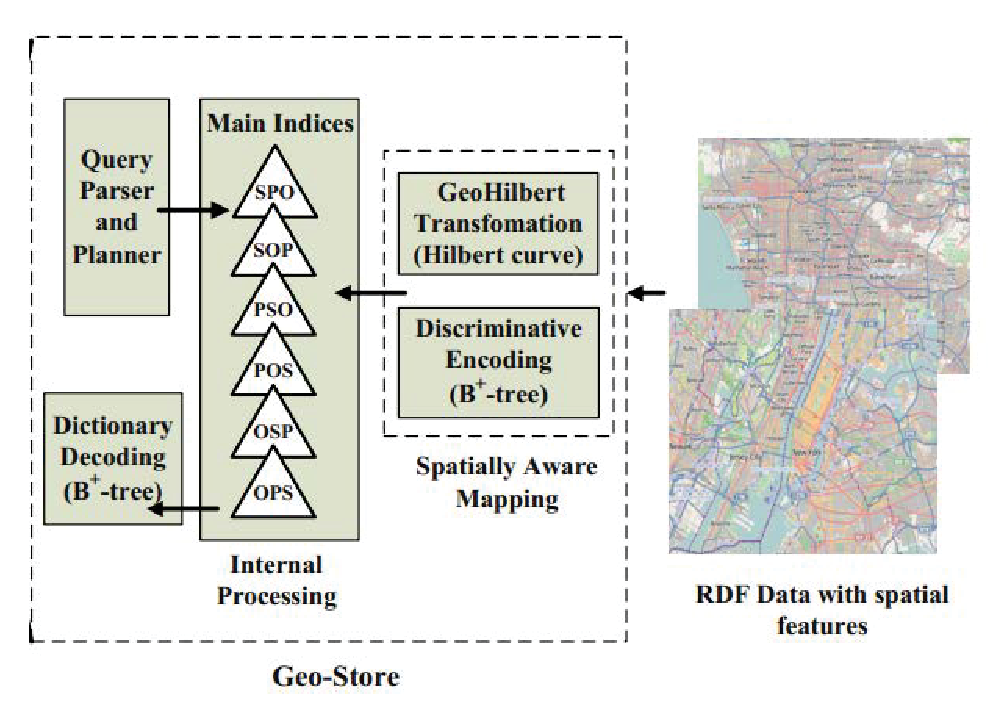
\includegraphics[width=3in]{images/architect.eps}
\caption{Geo-Store System Architecture}\label{fig:architect}
\end{figure}

\subsection{Spatial-Aware Hashing}

In order to support efficient geospatial query processing, the system performs spatial-aware hasshing (SAH) when geo-coordinates is encountered during insertion and update of data. The spatial-aware hasing is based on Hilbert space filling curve transformation, in which a two-dimensional coordinates of a point is transformed into an integer. A benefit of this transformation is to reduce a RDF geo-coodinates literal into a short integer; therefore, eliminating long string comparison during query evaluation. Another benefit is that the transformation produces locality-preserving results, so two points that are ``close" in the original space will have high chance of being hashed to close values. The query evaluator uses this locality-preserving property to approximate spatial extend of spatial constraints of a query.

The result of the a SAH is placed into the underlying data store as a triple, where the subject is the entity of which the location was hashed. The hashed value is then further indexed by B-Tree indexes (shown as Main Indices in Figure~\ref{fig:architect}) for fast look-up.

\subsection{Spatial Query Analyzer}

After the SAH has been performed on newly inserted data, the system can start evaluating queries. When a query is received, the query analyzer looks for spatial filters within the query. When a filter is found, the analyzer uses the same spatial-aware hashing algorithm, described previously, to find a list of spatial hash values (integers) covered by the filter. Since the underlying data store does not aware any spatial context and only understand standard SPARQL patterns, the query analyzer translates the list of hash values into query patterns and removes the translated spatial filter. All these steps essentially adds SPARQL graph patterns to approximate the entities that are covered by the query filter. For multiple query filters within a query, the process is the same for each, but the analyzer performs union for overlapping hash values.

\section{Spatial Queries}

\underline{\textbf{Window Filter}} \\
Window filter constraints the binding of a query variable to within a rectangular region defined by two corners. The follow query is an example.

\begin{verbatim}
SELECT ?name ?location
WHERE{
    ?e <name> ?name.
    ?e <coordinates> ?location.
    within(?location, 32.5955, -85.4909, 32.6122,
           -85.4739)
}
\end{verbatim}
%\caption{\small Skyline SQL Clause.
%\label{fig:skyline_sql}}

\underline{\textbf{Range Filter}} \\
Range filter constraints the binding of a query variable to a circular region a distance from a center.

\begin{verbatim}
SELECT ?name ?location
WHERE{
    ?e <name> ?name.
    ?e <coordinates> ?location.
    within(?location, 32.597178, -85.463086, 1500)
}
\end{verbatim}

\underline{\textbf{Nearby Filter}} \\
Range filter constraints the binding of a query variable to a circular region a distance from a center.

\begin{verbatim}
SELECT ?name ?location
WHERE{
    ?e <name> ?name. ?e <coordinates> ?location.
    nearby(?location, 32.607985, -85.481439, 3)
}
\end{verbatim}

\section{Query Builder}

Figure~\ref{fig:geostore_web} shows the query builder of the system. The interface consists of two parts. The top part is the query editor that allows the user to manually enter the query. Below the editor is the builder tool that assist the user to construct query graph patterns as well as geospatil query filters.

\begin{figure}[t]
\centering
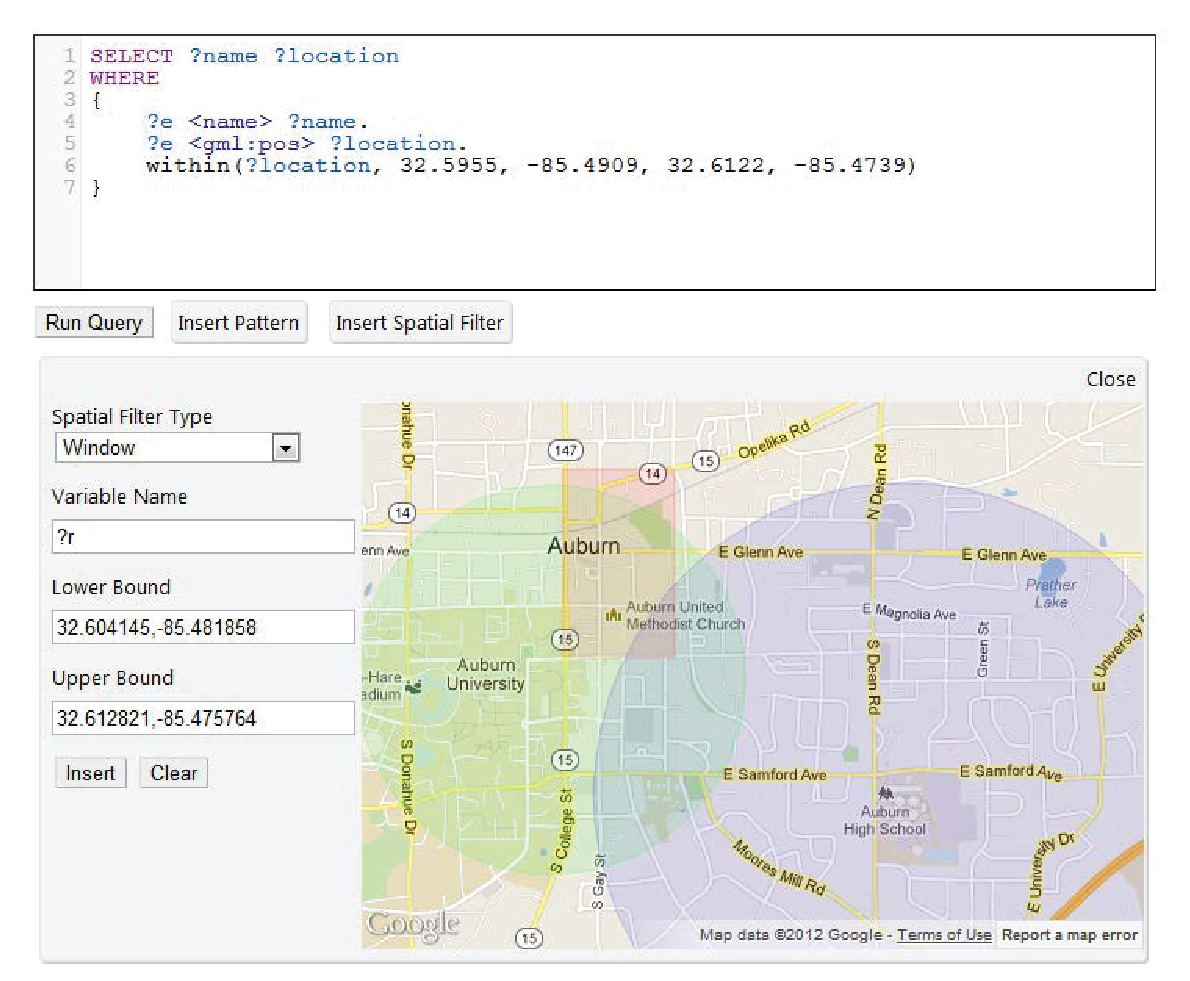
\includegraphics[width=3.3in]{images/geostore_web.eps}
\caption{Geo-Store Query Builder Interface}\label{fig:geostore_web}
\end{figure} 